%861
\newpage
\subsection{例題4-3 ミニサッカーゲームの動きを改造する}

\begin{description}
    \item \textgt{\bf 考え方}
\end{description}

ミニサッカーゲーム(kick.hsp)のプログラムを改造してゲームの内容を変えてみましょう。

このプログラムでは、変数を使って人の動きや、ボールの動きを計算しています。

変数の代入と計算の方法を覚えていますか?



プログラムの最初に、変数に値を代入しています。

この値を変更することで、ゲームの動きが大きく変わります。


\begin{figure}[H]
    \begin{center}
      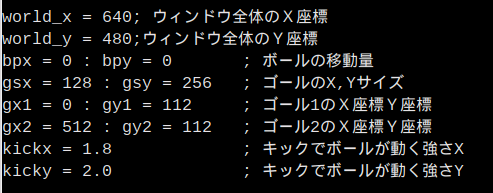
\includegraphics[keepaspectratio,width=13.044cm,height=5.106cm]{text04-img/text04-img010.png}
      \caption{ミニサッカーゲームのプログラム}
    \end{center}
    \label{fig:prog_menu}
\end{figure}


でたらめに書き直してもエラーになったり、処理が遅くなったりするので、あまり大きく変えないようにしましよう。

どの変数が、どのような働きをしているかをコメントとして書いてあります。


\begin{description}
    \item \textgt{\bf \ \ 変数 = 数字 \ \ \ \ \ \ \ \ \ \ \ \ \ \ \ \ \ \ \ \ \ \ \ \ \ \ \ \ \ \ \ \ \ \ ; コメント}
\end{description}

となっている時、「; コメント」の部分は、プログラムの実行には関係ないですがメモを残す意味で、文字が書かれています。「;」記号から後ろはコメントとして扱われるルールだということを覚えておきましょう。

Xは横方向の動きを表しています。Yは縦方向です。

数字を変えてどのように変わるか試してみましょう。


\begin{description}
    \item \textgt{\bf 例題4-3 答え}
\end{description}



「kickx = 1.8」の数字を少しだけ大きくしてみましょう。

(大きくしすぎないようにしてください)

「kicky = 2.0」なども変えてみると、どうなるか確認してみましょう。



[F5]キーを押して改造したゲームがきちんと動くか確認しましょう。

改造ができたらTAや周りの友達にも見せてあげましょう。









